\documentclass[a4paper]{article}

\usepackage{amsmath}
\usepackage{enumitem}

\usepackage{subfigure}
\usepackage{amsmath}
\usepackage{amssymb}
\usepackage{graphicx}

\usepackage[font=small,labelfont=bf]{caption}

\DeclareMathOperator*{\argmin}{arg\,min}
\author{Kennard Ng and Luo Wen Han}
\title{Project 2: Latent Dirichlet Allocation}

\bibliographystyle{unsrt}

\begin{document}
	\maketitle
	\section{Introduction}
	
	% todo change this to what we are trying to solve exactly. 
	In this project, we find the underlying population distribution of an individual by his genotype.
	We model the this problem using the Latent Dirichlet Allocation (LDA)~\cite{blei2003latent} graphical model. Given that inference and learning on the LDA is intractable, we use variational inference with the mean field assumption to perform approximate inference.
	
	\section{Background}
	
	\subsection{Latent Dirichlet Distribution}
	The Latent Dirichlet Allocation (LDA) is a generative probabilistic model for a collection  of discrete data proposed by Blei et al.~\cite{blei2003latent}. In the original paper, Blei et al. use LDA to model text corpora, where they represent documents as a random mixture over latent topics where each topic is further characterized by their word distribution. 
	
	\begin{figure}[ht]
		\centering
		\captionsetup{width=.8\linewidth}
		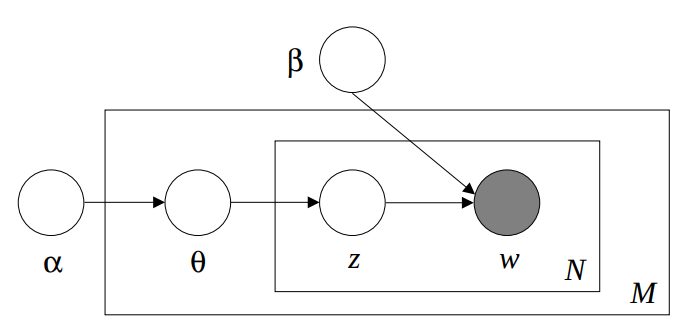
\includegraphics[width=0.6\linewidth]{images/lda_graphical}
		\caption{Graphical Model of LDA. Taken from~\cite{blei2003latent}. The plates represent replicas. In our context, the inner plate represents the repeated choice of ancestor populations and genotypes of a person while the outer plate represents the population with $M$ individuals.}
		\label{fig:ldagraphical}
	\end{figure}

	Similarly, we model a population's genetics by representing each individual as a mixture of his ancestor populations, where each ancestor population can be characterized by its distribution over the genotypes i.e. genetic data. We assume the following generative process for the genetic makeup of an individual:

	\begin{enumerate}[noitemsep]
		\item Assume that each individual has $N$ genotypes. 
		\item Choose $\theta \sim \mathrm{Dir}(\alpha)$.
		\item For each of the $N$ genotypes $w_n$:
		\begin{enumerate}
			\item Choose an ancestor population $z_n \sim \mathrm{Multinomial}(\theta)$.
			\item Choose a genotype $w_n$ from $p(w_n|z_n,\beta)$, where $p(w_n|z_n,\beta)$ is a multinomial distribution conditioned on the ancestor population $z_n$ and genotype prior $\beta$.
		\end{enumerate}
	\end{enumerate}
	
	\subsection{Variational Inference}
	
	During inference, we want to find the distributions over hidden variables $\theta, z$ given parameters $\alpha, \beta$ and observed variables $w$. We express this as the following posterior distribution:
	
	\begin{equation}
		p(\theta,z \mid w,\alpha,\beta) = \frac{p(\theta,z,w\mid \alpha,\beta)}{p(w\mid \alpha,\beta)}.
	\end{equation}
	
	\noindent Unfortunately, we see that exact inference is intractable given that the normalizer is intractable where
	\begin{equation}
		p(w | \alpha, \beta) = \int_{-\infty}^{\infty} \sum_{n=1}^N p(\theta,z_n,w\mid\alpha,\beta) d\theta.
	\end{equation}
	
	\noindent Hence, we make an approximate inference instead. We use the mean field assumption that assumes fully factorized distributions and we approximate the posterior distribution $p$ with an approximate distribution: 
	
	\begin{equation}
		q(\theta,z \mid \gamma,\phi) = q(\theta\mid\gamma) \prod_{n=1}^{N} q(z_n\mid\phi_n).
	\end{equation}
	
	\noindent The graphical model of our approximate distribution is given in Figure~\ref{fig:approximategraphical}.
	
	\begin{figure}[ht]
		\centering
		\captionsetup{width=.8\linewidth}
		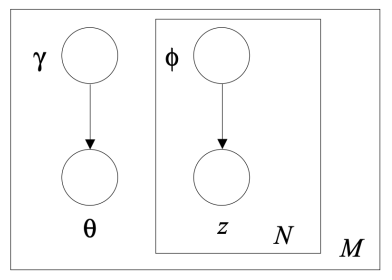
\includegraphics[width=0.5\linewidth]{images/approximate_graphical}
		\caption{Approximate Distribution under the Mean Field Assumption.}
		\label{fig:approximategraphical}
	\end{figure}
	
	
	\clearpage
	\bibliography{references.bib}
\end{document}